
%(BEGIN_QUESTION)
% Copyright 2011, Tony R. Kuphaldt, released under the Creative Commons Attribution License (v 1.0)
% This means you may do almost anything with this work of mine, so long as you give me proper credit

Determine how you would connect a hand pump and test gauge to the following level alarm system in order to test the alarm switch (LSH-37) to see if the alarm activates at its trip point of 11.5 feet:

$$\includegraphics[width=15.5cm]{i03449x01.eps}$$

\begin{itemize}
\item{} Identify the necessary tube connections to connect the pump and test gauge to LSH-37.
\item{} Calculate the proper amount of pressure to apply to the switch to make it ``think'' the transmitter is measuring 11.5 feet of liquid level
\end{itemize}

\underbar{file i03449}
%(END_QUESTION)





%(BEGIN_ANSWER)

5 points for correct connections ({\bf Transmitter output tube disconnected, pump and gauge connected to switch input port ``I''}), and 5 points for pressure value of {\bf 13.62 PSI}.

\vskip 10pt

-2 points if gauge and pump are connected to switch properly, but the level transmitter is still connected as well.

%(END_ANSWER)





%(BEGIN_NOTES)

{\bf This question is intended for exams only and not worksheets!}.

%(END_NOTES)


